\clearpage

\section{Analyse av opprinnelig løsning}

Målet med å analysere det nåværende nettstedet til Sirkus Media er å kartlegge eventuelle problemerområder som burde forbedres. Når utviklingen av det nye nettstedet er ferdig, vil vi sammenligne de nye testresultatene med resultatene som blir presentert i dette kapittelet.


\subsection{Test med Google Lighthouse}
\label{sec:analysis-current-lighthouse}

Ved å kjøre Google Lighthouse får vi resultater for hastighet, tilgjengelighet, beste praksis, søkemotoroptimalisering og progressiv webapplikasjon. Figur \ref{fig:analysis-current-lightouse-summary} viser oppsummering av resultatetene etter å ha kjørt testen. Oversikten viser at nettstedet får gode poeng på alle områdene. Dette fordi dagens nettsted består av kun en forside og lite informasjon. Dette begrenser muligheten for feil.

\begin{figure}[H]
    \centering
    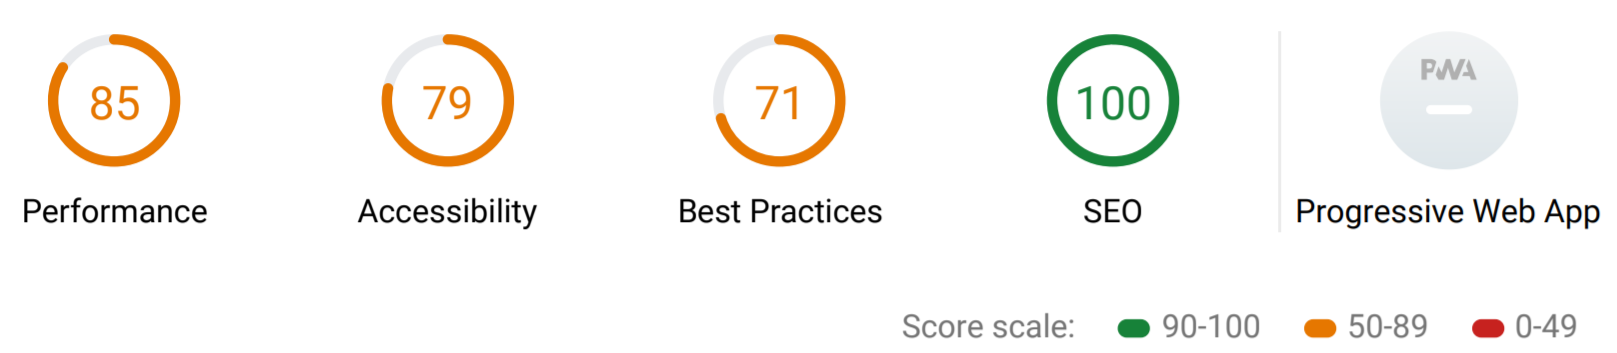
\includegraphics[width=\textwidth]{bjornar/Lighthouse Report - mobile.png}
    \caption{Resultater fra Google Lighthouse}
    \label{fig:analysis-current-lightouse-summary}
\end{figure}


Ikonet for \q{Progressive Web App} har en feil, slik at man ikke får sett scoren. Ved hjelp av en JSON-fil \footnote{Se JSON-fil, linje 3386} som inneholder resultatene, ser man at poengscoren er på 58\%.


\subsection{Checkbot}
Checkbot \footnote{https://checkbot.io} tester sikkerhet, hurtighet og søkemotoroptimalisering. Figur \ref{fig:analysis-current-checkbot-summary} viser oppsummering av resultatet. En mer detaljert rapport kan leses under vedlegg X. Denne testen viser en god poengsum når det gjelder totalt for gjennomsnittet. Isolert sett ser vi at sikkerheten til nettstedet drar ned poengscoren betydlig.

\begin{figure}[H]
    \centering
    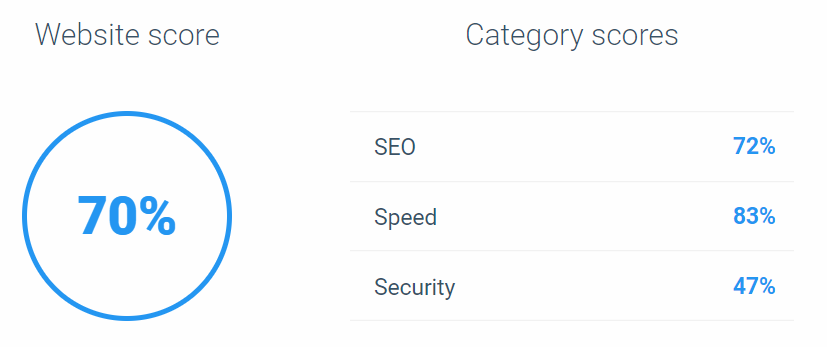
\includegraphics[width=0.75\textwidth]{bjornar/checkbotio-summary.png}
    \caption{Checkbot.io summary}
    \label{fig:analysis-current-checkbot-summary}
\end{figure}



\subsection{Color Contrast Analyzer}

Kan lastes ned her
\url{https://chrome.google.com/webstore/detail/color-contrast-analyzer/dagdlcijhfbmgkjokkjicnnfimlebcll}

Lagd av
\url{https://accessibility.oit.ncsu.edu/} (North Carolina State University)

Verktøyet tar bilde av nettstedet og scanner deretter kontrasten. Områder med bedre kontrast utheves og får lyse kanter. Jo mer markante kanter, desto mer kontrast.

\begin{figure}[H]
    \centering
    \makebox[\textwidth]{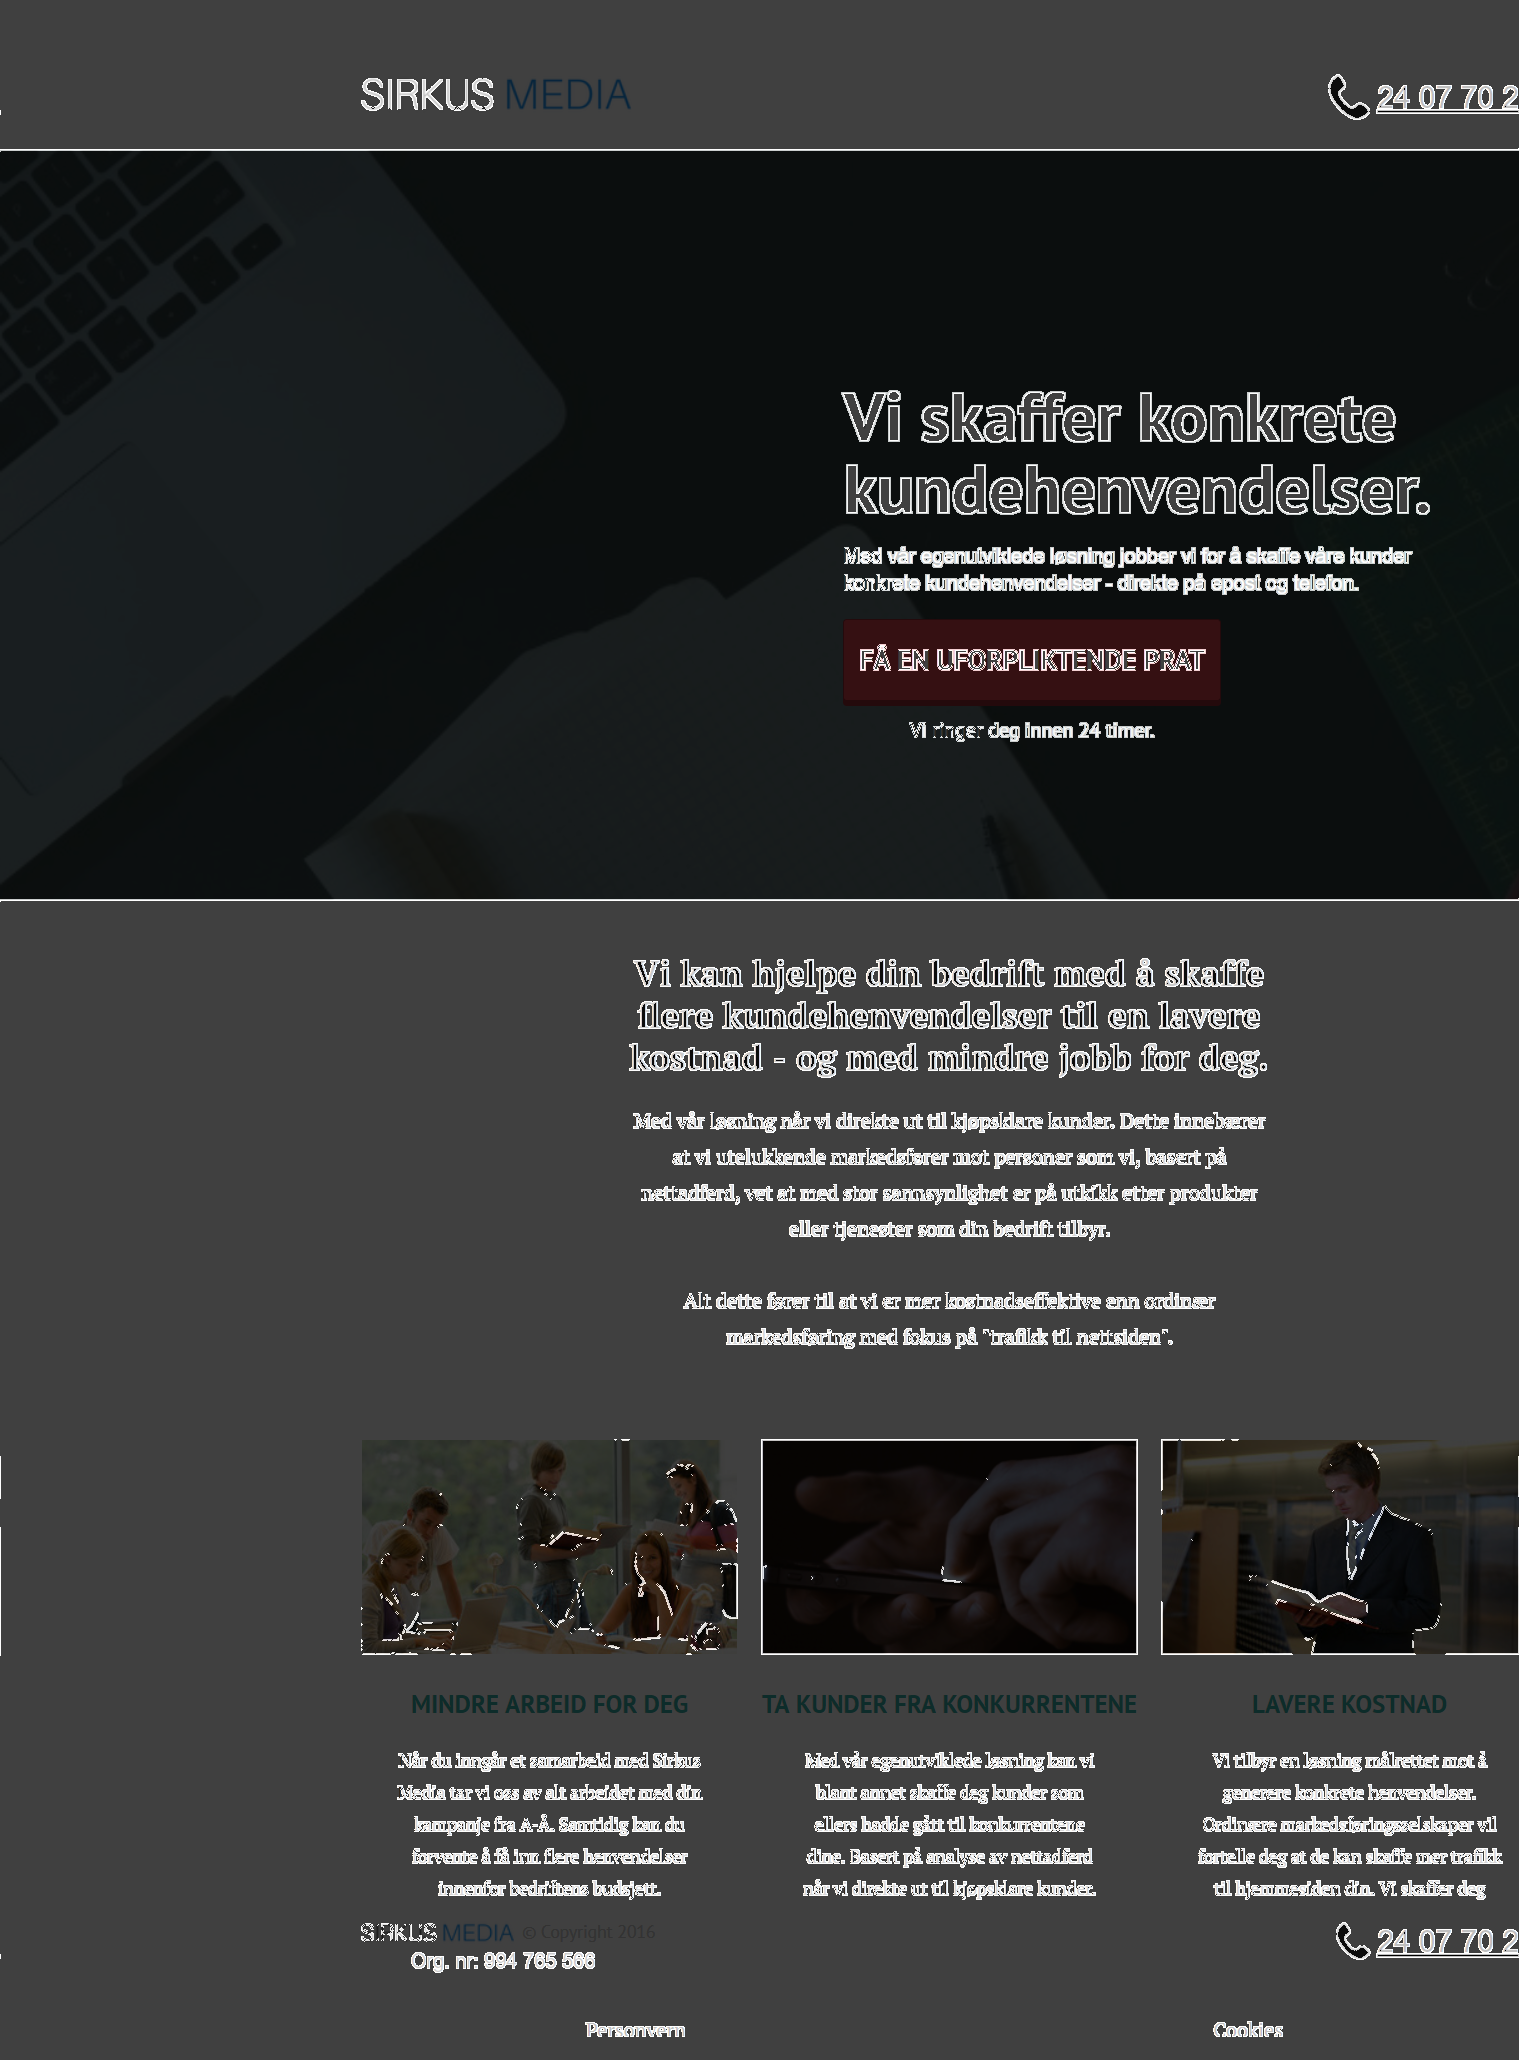
\includegraphics[width=0.80\paperwidth]{bjornar/contrast-wcag-aa-small.png}}
    \caption{CCA resultat AA}
    \label{fig:analysis-current-cca-aa}
\end{figure}

\begin{figure}[H]
    \centering
    \makebox[\textwidth]{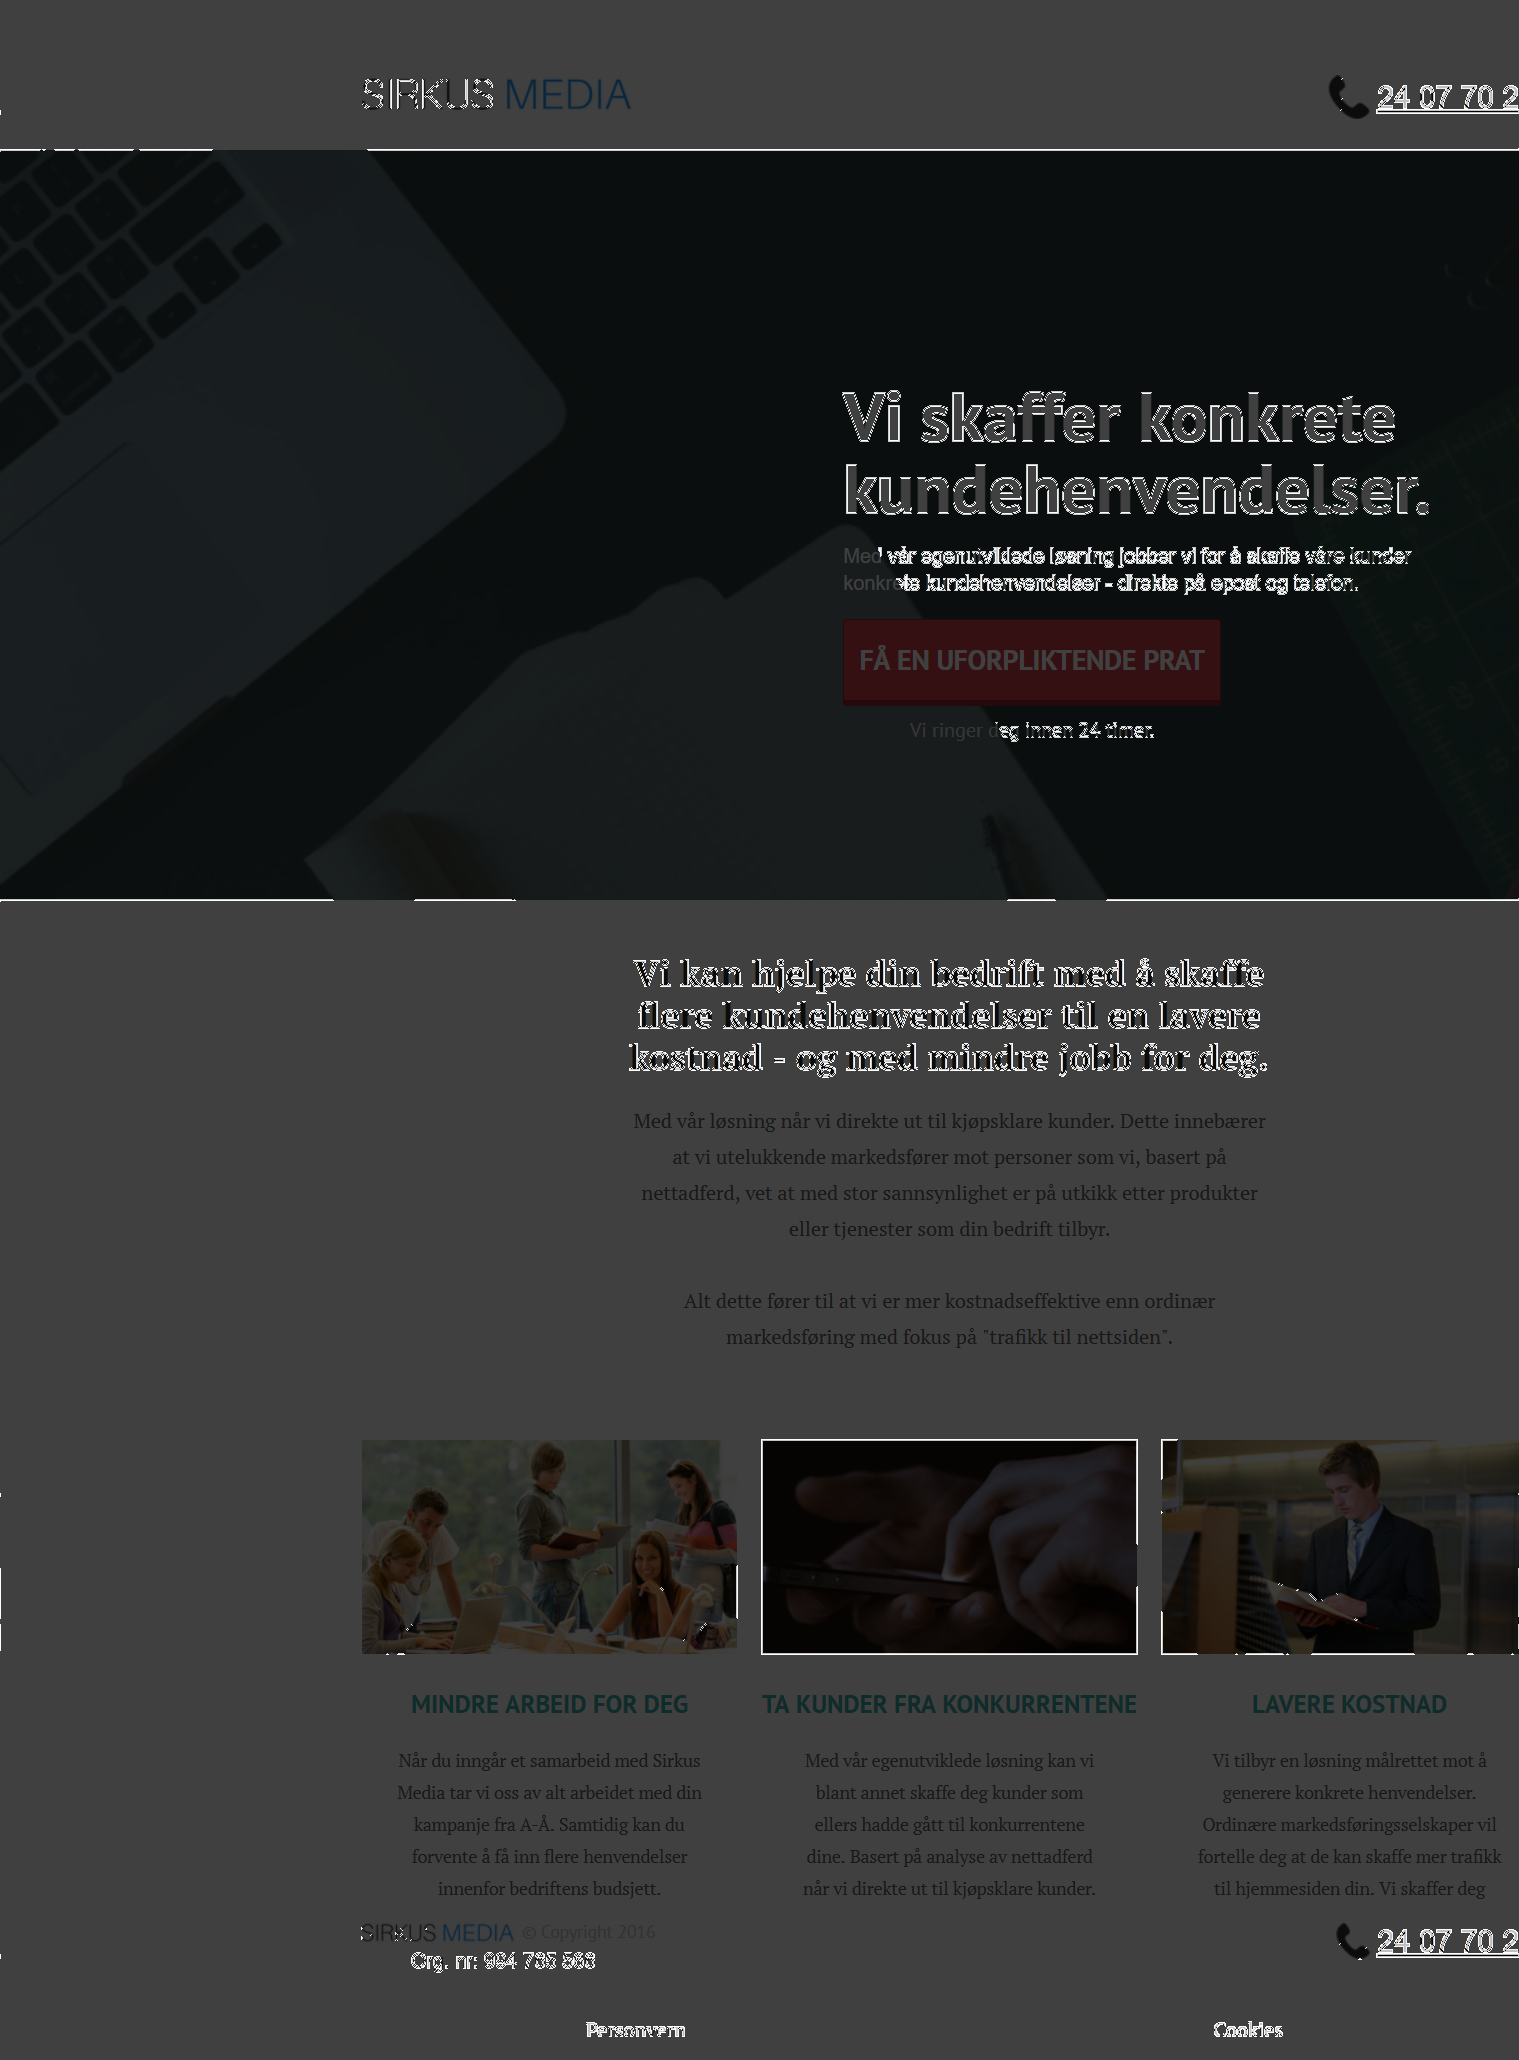
\includegraphics[width=0.80\paperwidth]{bjornar/contrast-wcag-aaa-small.png}}
    \caption{CCA resultat AAA}
    \label{fig:analysis-current-cca-aaa}
\end{figure}

Ved å kjøre testen \q{small non bold text} for nivå AA, som gjelder for skriftstørrelser opptil 18pt, viser resultatene at deler av teksten i logo og de grønne overskriftene ikke har gode nok kontraster. Dette illustreres i figur \ref{fig:analysis-current-cca-aa}. Chrome DevTools verifiserer at kontrastforholdet ikke oppfyller kontrastkravet for AA. Se figur \ref{fig:analysis-current-cdt-a} og \ref{fig:analysis-current-cdt-b}

\begin{figure}[H]
    \begin{center}
        \subfigure[grønn overskrift]{\label{fig:analysis-current-cdt-a}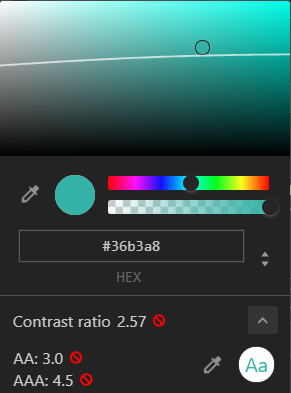
\includegraphics[width=0.3\textwidth]{bjornar/contrast-wcag-aa-small-gronn-tekst.png}}
        \subfigure[blå logo tekst]{\label{fig:analysis-current-cdt-b}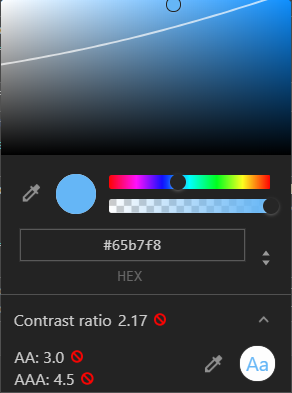
\includegraphics[width=0.3\textwidth]{bjornar/contrast-wcag-aa-small-logo-blaa.png}}
        \subfigure[body tekst]{\label{fig:analysis-current-cdt-c}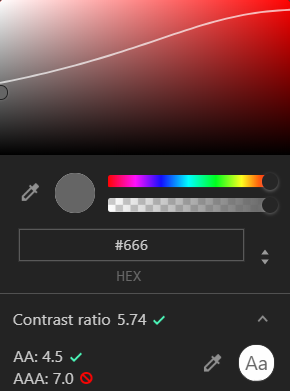
\includegraphics[width=0.3\textwidth]{bjornar/contrast-wcag-aaa-small-body.png}}
        \caption{Chrome DevTools - color a11y}
        \label{fig:analysis-current-cdt}
    \end{center}
\end{figure}

Resultatene etter å ha kjørt tester for nivå AAA viser at mesteparten av nettstedet ikke oppfyller kravet for kontrastnivå. Se figur \ref{fig:analysis-current-cca-aaa}. Her blir ingen av avsnittene med ordinær skriftstørrelse markert. Ved å kjøre en test med Chrome DevTools verifiseres påstanden om for dårlig kontrastnivå. Se figur \ref{fig:analysis-current-cdt-c}.


\subsection{WAVE}
\url{http://wave.webaim.org/}

Kan videre \q{verifisere} funnene som ble gjort med verktøy over (CCA)r. LAG REF.

Ved å skru på \q{No-styling} vil man oppdage at det er en skjult seksjon på siden.
\q{THE COMPANIES THAT MAKE THEIR LIFE SIMPLE}. Dette blir plukket opp av skjermlesere og er derfor ikke ideelt.

Det ble også oppdaget andre feil:
1x: Document language missing
4x: Tomme linker
5x: Redudante linker

Annet:
8x: Bilder med tom alt attr.

Bra stuktur på overskrifter som følger beste praksis:
\begin{itemize}
    \item h1: Vi skaffer konkrete kundehenvendelser.
    \begin{itemize}
        \item h2: Vi kan hjelpe din bedrift med å skaffe flere kundehenvendelser til en lavere kostnad - og med mindre jobbe.
        \begin{itemize}
            \item h3: MINDRE ARBEID FOR DEG
            \item h3: TA KUNDER FRA KONKURRENTENE
            \item h3: LAVERE KOSTNAD
        \end{itemize}
    \end{itemize}
\end{itemize}

\subsection{Bakgrunnsbilde A11y test}
\url{https://www.brandwood.com/a11y/}

Ved å se på resultatene som ble presentert etter å ha benyttet CCA kan det konkluderes med at kontrastene er gode nok for nivå AA, men at de ikke oppfyller kravene for AAA. Dette er vanskelig å få verifisert med Chrome DevTools eller WAVE. Begge disse verktøyene kan gi negative resultater som er falske ettersom de ikke får en bakgrunnsfarge å se på, men et bakgrunnsbilde. Dette fører til at testen ikke blir utført korrekt.

For å forhindre dette kan Brandwood sin A11y-test benyttes. Verktøyet deler opp bilde, der det ligger tekst over, i seksjoner og finner gjennomsnittsfargen i hver seksjon. Deretter sjekkes kontrastforholdet mellom hver seksjon og teksten.
Se figur.

\begin{figure}[H]
    \centering
    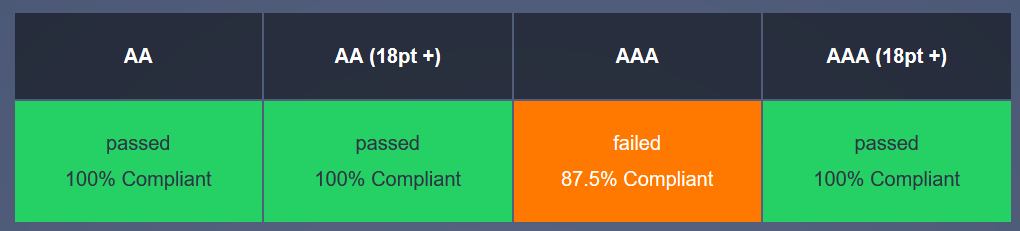
\includegraphics[width=\textwidth]{bjornar/bg-image-h1.png}
    \caption{heading tekst}
    \label{fig:analysis-current-a11y_bg-h1}
\end{figure}

\begin{figure}[H]
    \centering
    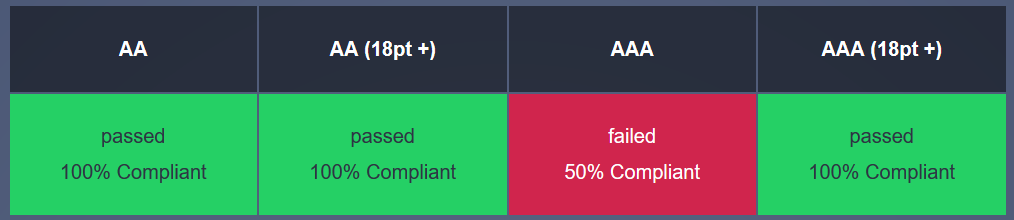
\includegraphics[width=\textwidth]{bjornar/bg-image-p.png}
    \caption{p tekst}
    \label{fig:analysis-current-a11y_bg-p}
\end{figure}

\begin{figure}[H]
    \centering
    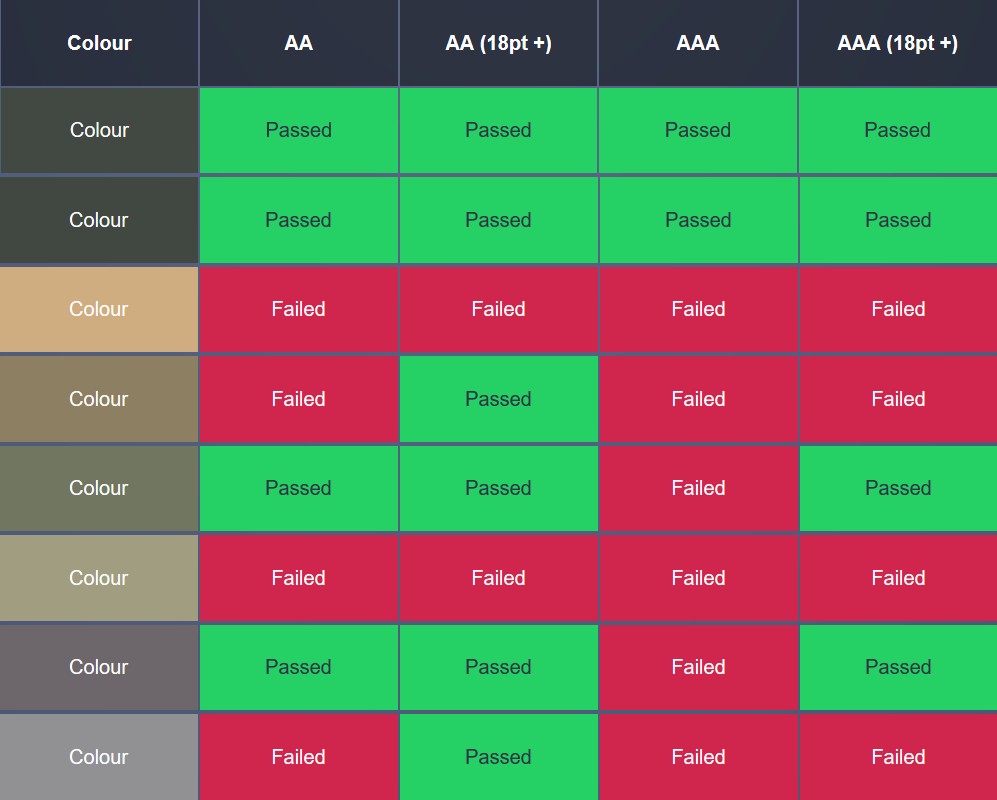
\includegraphics[width=\textwidth]{bjornar/bg-image-eksempel.png}
    \caption{Eksempel}
    \label{fig:analysis-current-a11y_bg-example}
\end{figure}


\subsection{Chrome DevTools}

Chrome DevTools kan brukes til å sjekke kontrastforhold.

Nettverksfanen kan sjekke hastighet.
Gjennomsnitt:\\
- DOM: 417ms\\
- Load: 1392ms

\begin{table}[H]
\begin{tabular}{lllll}
Test & DOM & Load &  &  \\
1 & 398 & 1250 &  &  \\
2 & 501 & 1640 &  &  \\
3 & 422 & 1420 &  &  \\
4 & 387 &  928 &  &  \\
5 & 375 & 1720 &  & 
\end{tabular}
\end{table}

Resultatene måles i millisekunder. Testene ble kjørt på nettverket til Høgskolen i Østfold (avdeling Halden) fra en Dell XPS 13 (9350)

\subsection{GOOGLE TRANSPARENCY REPORT - Safe Browsing: malware and phishing}
\url{https://transparencyreport.google.com/safe-browsing/search?url=https://sirkusmedia.no&hl=en-US}

Det ble også gjort tester for å sjekke om det var skadevare på siden.
Ingen funn ble gjort her, noe som selvfølgelig er positivt.

\subsection{SSL test}

\url{https://www.ssllabs.com/ssltest/}

Resultatet ble en A. Dette er bra, men nettstedet burde fått det beste resultatet som er A+, da det hverken kreves mye tid eller ressurser for å oppnå dette.

\begin{figure}[H]
    \centering
    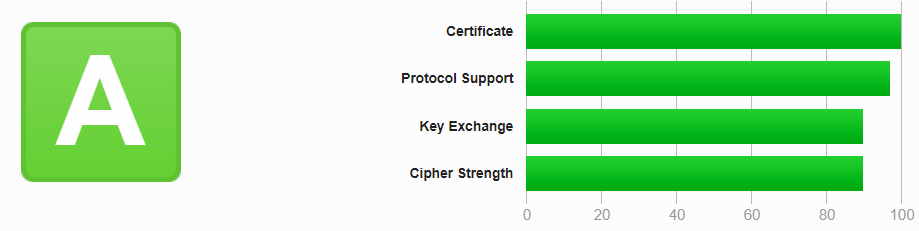
\includegraphics[width=\textwidth]{bjornar/ssllabs.png}
    \caption{Sertifikat score}
    \label{fig:analysis-current-ssl}
\end{figure}


\clearpage